\chapter{Python's threading model}
\label{cpt:pythons_thread_model}

Before we can address Tribler's blocking I/O problem, we first need to better understand Python's threading model and how the Python interpreter behaves.
By looking in depth how the operating system (OS) and the python interpreter behave together, how threads run concurrently and the pros and cons of concurrency, we can look into if asynchrony can boost Tribler's performance.
This allows us to answer the second research question \enquote{Can a system such as Tribler benefit from asynchrony?} and gives us a direction of design and implementation.

\section{Threads in Python}

\begin{figure}[!h]
	\makebox[\textwidth][c]{\includegraphics[width=\linewidth]{pythonthreading/diagrams/thread_io_release_diagram}}
	\caption{A schematic view of how threads release the GIL when performing IO in Python.}
	\label{fig:python_threads_release_gil}
\end{figure}

Python threads are normal OS threads, either POSIX (pthread) or Windows threads \cite{beazley2010understanding, beazley2009inside}.
Python does not feature a thread scheduler, threads are fully managed by the operating system that hosts them.
To control thread execution Python features a construct called the Global Interpreter Lock (GIL).
This GIL ensures that only one thread can run in the python interpreter at once, i.e. a thread needs to hold the GIL in order to execute.
This means there cannot be any parallel execution.
Once a thread is done executing or needs to block it releases the GIL.
This gives way for cooperative multitasking as other threads that are ready to execute can try to acquire the GIL, visualized in Figure \ref{fig:python_threads_release_gil}.

To make sure Central Processing Unit (CPU) bound tasks do not hold the GIL indefinitely a simple check mechanism is built in that \enquote{checks} every thread once per 100 ticks.
Ticks are loosely mapped to interpreter instructions and do not define a time unit.
Listing \ref{lst:one_tick} contains two code samples that only take one tick each, but take require different amount of time to compute.

\lstinputlisting[caption={Two code samples that each take one tick yet require a different amount to compute.},label={lst:one_tick},language=Python]{pythonthreading/code/one_tick.py}

When a check is run the following four steps are executed:
\begin{enumerate}
	\item The thread that holds the GIL resets its tick counter.
	\item If the current thread it the main thread, it runs the signal handlers.
	\item The thread releases the GIL.
	\item The thread tries to reacquire the GIL.
\end{enumerate}

Note that a thread may immediately reacquire the GIL after releasing it.
Since every thread has this check, CPU-bound threads will engage in cooperative multitasking.

\section{Multi threaded programming performance}
\label{sct:multi_theaded_programming_performance}

\begin{table}[h]
	\centering
	\begin{tabular}{l|l}
		\textbf{Component} 	& \textbf{Specifications} \\ \hline
		Operating System   	& Ubuntu 16.04 LTS \\
		Python version		& 2.7.12 \\
		CPU					& Intel Core i5-2410M \\ 
		HDD					& Samsung 850 EVO 250GB  \\ 
		RAM					& 8 GB DDR3 1600MHz \\
	\end{tabular}
	\caption{Specifications of the setup used during the rerun David Beazly's experiment.}
	\label{table:rerun_beazily}
\end{table}

Because threads cannot run in parallel, this changes the performance one may expect from a multi-threaded program.
Dadiv Beazly presented his findings in his Python Concurrency Workshop (2009) \cite{beazley2009inside}.
By running a trivial CPU-bound function using two threads on a dual-core MacBook, processing time increased 24.6 to 45.5 seconds; an increase of 185\%.
Disabling one of his cpu cores yielded 38.0 seconds, an increase of 154\% in run time.

To confirm this behaviour still exists in the latest version of Python2, we rerun Beazly's experiment.
The setup used in this experiment can be found in Table~\ref{table:rerun_beazily}.
Running it sequentially gives us a run time of 8.17 seconds, whereas running it using two threads provides us with a run time of 14.49 seconds; an increase of 177\% which is in range of Beazley's observations

To investigate this behaviour, Beazley studied the underlying C code to inspect why he was observing these performance results.
Whenever a (Python) thread releases the GIL, it sends out a signal.
The OS then propagates this signal to other threads which then can attempt to acquire the GIL.
The time or \emph{lag} between thread switching and execution may be significant depending on the OS, according Beazley.
Most operating systems make use of a priority system for threads: the thread with the highest priority will be scheduled by the OS.
Often, CPU-bound threads have a low priority and I/O-bound threads a high priority.
If a signal is send to a low priority thread and all CPUs are currently busy processing other, high priority threads, it won't be run until one of the CPUs becomes available.

As it turns out, the GIL signalling is the source of the performance loss.
Whenever the periodic \enquote{check} runs, the following happens:

\begin{itemize}
	\item First the Python interpreter locks a mutex.
	\item Next, it signals on a condition variable/semaphore where another thread is \emph{always} awaiting execution.
	\item Because of this waiting thread, additional pthread processing and system calls are generated to deliver the signal.
\end{itemize}

Beazley provided rough measurements on the number of system calls generated, summarized in Table~\ref{tbl:system_calls_thread_switching}.
From these numbers Beazley concludes that the amount of additional calls generated is significant and the main reason for the performance loss.
He then dived deeper into these numbers to find a cause.

 \begin{figure}[h]
 	\makebox[\textwidth][c]{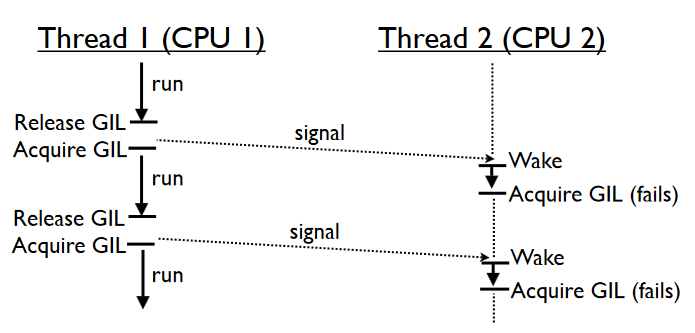
\includegraphics[width=\linewidth]{pythonthreading/images/gil_battle_threads}}
 	\caption{A schematic view of two threads battling for GIL acquisition (source: David Beazley, 2009).}
 	\label{fig:gil_battle_threads}
 \end{figure}

By recording a real-time trace of all GIL related operations i.e. acquisition, release, etc., Beazley was able to reconstruct the key problem.
When running multiple CPU-bound threads on multiple cores, all of them will be scheduled \emph{simultaneously}.
The threads proceed to battle over GIL acquisition. 
Whenever a thread releases the GIL because of the 100 tick \enquote{check}, it immediately tries to reacquire it.
Another thread will also try to acquire the GIL upon this signal, but as this signal arrives with a delay it will most likely fail.
This processes is visualized by Figure~\ref{fig:gil_battle_threads} (David Beazley, 2009).
Beazley argues that here two competing goals are clashing.
On the one hand Python wants to only run one thread at a time where on the other hand the OS wants to schedule as many processes/threads to take advantage of its multiple core architecture.
This clash raises a lot of overhead, which results in a severe performance penalty.

Even running threads on one core result in these GIL acquisition battles.
I/O-bound threads which are high priority may fail to acquire the GIL when a CPU-bound thread is busy, degrading the response time of the I/O thread.

\begin{table}[]
	\centering
	\begin{tabular}{|l|l|l|l|}
		\hline
	\textbf{Threads}	& \textbf{Cores} & \textbf{Unix system calls} & \textbf{Mach system calls} \\ \hline
	1	& 1 & 736 & 117 \\ \hline
	2	& 1 & 1149 & 3.3M \\ \hline
	2	& 2 & 1149 & 9.5M \\ \hline
	\end{tabular}
	\caption{A summary of the measurements from David Beazley \cite{beazley2009inside}.}
	\label{tbl:system_calls_thread_switching}
\end{table}

\subsection{A new GIL}

To solve the excessive amount of GIL signalling, a new GIL has been introduced in Python 3.2 \cite{beazley2010understanding}.
Instead of having the 100 ticks \enquote{check}, there is now a global variable.
A thread will continue running until this variable is set to one (1), indicating another thread requests to acquire the GIL at which the running thread must release the GIL.
This means whenever only one thread is running, the variable will never be set (there is no competing thread) and no signalling takes place.
Whenever another thread is present, it will be in a suspended state as it does not hold the GIL, and starts a five millisecond timeout.
From here two things can happen: the running thread releases the GIL voluntarily within the timeout (e.g. an I/O operation is performed) at which the other thread can immediately acquire it, or the timeout expires.
If the timeout expires, the other thread will set the global variable to one and enters another timeout, awaiting a signal that the GIL has been released.
The running thread will release the GIL, sends out a signal that it has done so and starts a wait period.
When the other thread acquires the GIL it will send out an acknowledgement to the thread that just released the GIL and starts its computations.
Finally, the former running thread will now enter a timeout upon receiving the acknowledgement so that it may require the GIL again.

To observe if the new GIL has any better performance, Beazley ran the same experiment using Python 3.2 and the results look promising.
Running the code sequentially, using two threads and using four threads on a quad core MacBook resulted in run times of 11.53, 11.93 and 12.32 second respectively.
Unfortunately, there are caveats when performing I/O operations using the new GIL.
Whenever an I/O operation does not block, the thread still releases the GIL which requires the thread to initiate the timeout again to reacquire the GIL.
Meanwhile CPU bound threads will also attempt to acquire the GIL since it was released, causing stalls.
Beazley argues that some more work is required on the GIL to get rid of this behaviour, yet expresses that even with the GIL present threads can still deliver excellent performance and programmers still should use threads when appropriate.

Unfortunately, Tribler currently runs on Python 2.7 and a considerable amount of work is required to migrate to Python3.
However, as the new GIL does look promising with respect to blocking I/O it can be noted down as an item for future work.

\section{Attempts to parallelize Python}
\label{sct:removing_the_gil}

Parallelize Python by removing the GIL and other means to speed up Python are topics that regularly return in the Python mailing list and at PyCon \cite{python2015global}.
Throughout the years many attempts have been made to alter Python or remove the GIL to fully benefit from multiple CPUs.
To date, no one has succeeded in removing the GIL and meet the (hard) requirements for replacement \cite{python2015global}.

On of the most well-known alternative implementations of Python is PyPy.
It makes use of a tracing Just-in-Time compiler to produce optimized code \cite{bolz2009tracing}.
By doing so, PyPy offers increased speed, reduced memory usage and support for stackless mode while providing a high compatibility with existing python code \cite{pypy2016pypy}.
PyPy's geometric average is 7.6 times faster than CPython (normal Python) \cite{pypy2016speed}.
While it has many popular libraries ported to be used with PyPy, it still lacks some common used packages.
Moreover, most of these libraries are not available on the official packaging repositories of Ubuntu and/or Debian, rendering PyPy unusable for the Tribler project as publishing Tribler on said repositories requires the dependencies to be available on them as well.

Two other popular implementations are JPython and IronPython.
Both these projects have removed the GIL and can fully exploit multiprocessor systems \cite{python2015global}.

JPython is a Python interpreter implemented in Java. It can be integrated in Java applications and allows python applications to be compiled into Java classes.
Using JPython, Python after compiled to java bytecode will run in the Jython virtual machine, giving full access to all Java APIs and classes \cite{jython2016why}.

IronPython does basically the same as JPython, compiling the source to in-memory bytecode and runs it on the Dynamic Language Runtime \cite{ironpython2014}.
It allows developers to run Python using the .NET framework.

To illustrate the attempts to remove the GIL are still on going, Larry Hastings presented \enquote{The Gilectomy} at PyCon 2016.
He showed that removing the GIL is fairly easy, but has a huge negative impact on CPython's performance, cache misses being the main reason.
Additionally, Hastings names some methods that may make The Gilectomy a viable alternative to CPython.\\

Libraries that introduce parallelism or asynchrony to gain performance are also available in large numbers.
In particular, many projects exist that attempt to make I/O asynchronous \cite{asyncio2016python}.
Often, these leverage the multiprocessing package in the standard library of Python.

Decorated Concurrency (DECO) uses the multiprocessing package of Python to parallelize functions using a \enquote{concurrent} decorator \cite{sherman2016deco}.
Different processes have their own Python interpreter which in turn has its own GIL, which allows for parallel processing.
Using the \enquote{concurrent} decorator, a function will be wrapped and executed on a new process.
Similarly, the \enquote{synchronized}  inserts synchronization events to automatically refactor assignments of the results of \enquote{concurrent} function calls to happen during synchronization events.
However, because of the overhead creating a new process generates and communicating between different processes, this approach is only viable for heavy loads that generally can run on its own.
The authors mention that a function should at least have an execution time of one millisecond for this method to be beneficial.

\section{Asynchronous programming}

\begin{figure}[!h]
	\makebox[\textwidth][c]{\includegraphics[width=0.6\linewidth]{pythonthreading/diagrams/normal_execution_flow}}
	\caption{Synchronous processing of tasks}
	\label{fig:normal_execution_flow}
\end{figure}

\begin{figure}[h]
	\makebox[\textwidth][c]{\includegraphics[width=0.6\linewidth]{pythonthreading/diagrams/delays_in_execution}}
	\caption{Tasks will be waiting when disk or network has to catch up.}
	\label{fig:delays_in_execution}
\end{figure}

A second option it to make use of asynchronous programming to gain performance.
Traditionally, synchronous programs execute tasks one by one as visualized in Figure\ref{fig:normal_execution_flow}.
When these functions perform an I/O operation, they are waiting for the disk or network to catch up, visualized in Figure~\ref{fig:delays_in_execution}.
In turn, the thread these functions run on will block, see Figure~\ref{fig:normal_io_flow}.
This means the main thread of a program will block if the I/O call happens on that thread.
A synchronous program that performs I/O operations regularly will therefore spend much of its time blocked waiting for disk or network to catch up.

\begin{figure}[t]
	\centering
	\begin{subfigure}[b]{\textwidth}
		\includegraphics[width=\textwidth]{problemDescription/images/normal_io_flow.png}
		\caption{A schematic overview of an I/O operation done by the main thread (synchronous).}
		\label{fig:normal_io_flow}
	\end{subfigure}
	~ %add desired spacing between images, e. g. ~, \quad, \qquad, \hfill etc. 
	%(or a blank line to force the subfigure onto a new line)
	\begin{subfigure}[b]{\textwidth}
		% To not scale this picture, the width of the normal flow image is 755, this one 595, hence a ratio of 0.79
		\includegraphics[width=0.79\textwidth]{problemDescription/images/async_io_flow.png}
		\caption{A schematic overview of an I/O operation executing on a separate thread, retuning a deferred (asynchronous).}
		\label{fig:async_io_flow}
	\end{subfigure}
	\caption{A schematic overview of a how an I/O call is handled in a synchronous versus an asynchronous manner.}
\end{figure}

In asynchronous programming, tasks are split into multiple chunks and executed interleaved, see Figure~.
The fundamental idea behind this approach is that when faced with a task that would normally block waiting for I/O, it will instead execute some other task that can still make progress.
This approach can outperform a synchronous program dramatically.

Support for asynchrony in python 2.7 is poor so the use of a framework is required.
Tribler makes use of Twisted, an event-driven networking engine written in Python \todo{cite naar Twisted pagina} which allows for event-driven and asynchronous programming. 

When programming asynchronously in Twisted, the function that is being called (callee) returns a deferred.
A deferred is a place holder for the actual value that the callee eventually will return once its done computing.

To ensure I/O operations does not block the main thread, the I/O can be moved to a separate thread, returning a deferred.
By attaching a callback and an errback, the caller can handle the case of a success and failure respectively.
These callbacks are handled by Twisted's event loop.
This thread can then block while the main thread continues executing other scheduled task.
Once the thread is done with its task it can invoke the callback of the deferred, notifying Twisted's event loop.
The event loop will then schedule the continuation of the previous task and proceeds executing the current task if not done yet, see Figure~\ref{fig:async_io_flow}.

\subsection{Drawbacks}

The main drawback of asynchronous programming is that it theoretically makes the structure more complex.
As any task can run while another task is waiting, one must be careful that the current task does not modify information the waiting task is dependant on.
Especially when working with databases one needs to make sure that the order of database queries is not different.

A second point of attention is the overhead generated when creating multiple threads.
As pointed out by the previous sections, offloading work to multiple threads may actually have a negative impact on performance.

\subsection{Initial measurements}

\begin{table}[h]
	\centering
	\begin{tabular}{l|l}
		\textbf{Component} 	& \textbf{Specifications} \\ \hline
		Operating System   	& Ubuntu 15.10 \\
		Python version		& 2.7.11 \\
		CPU					& Intel Core i7-2630QM \\ 
		HDD					& Samsung 850 EVO 500GB  \\ 
		RAM					& 8 GB DDR3 1600MHz \\
	\end{tabular}
	\caption{Specifications of the setup used in the initial CPU/IO/Network experiment}
	\label{table:setup_initial_experiment}
\end{table}

\begin{table}[]
	\centering
	\begin{tabular}{|c|c|c|c|}
		\hline
		\textbf{Configuration}	& \textbf{I/O Asynchronous} & \textbf{CPU Asynchronous} & \textbf{Network Asynchronous} \\ \hline
		0	& no & no & no \\ \hline
		1	& yes & no & no \\ \hline
		2	& no & no & yes \\ \hline
		3	& yes & no & yes \\ \hline
		4	& no & yes & no \\ \hline
		5	& yes & yes & no \\ \hline
		6	& no & yes & yes \\ \hline
		7	& yes & yes & yes \\ \hline
	\end{tabular}
	\caption{Overview of which workload is processed asynchronously per run configuration.}
	\label{tbl:experiment_configuration}
\end{table}

\begin{figure}[h]
	\makebox[\textwidth][c]{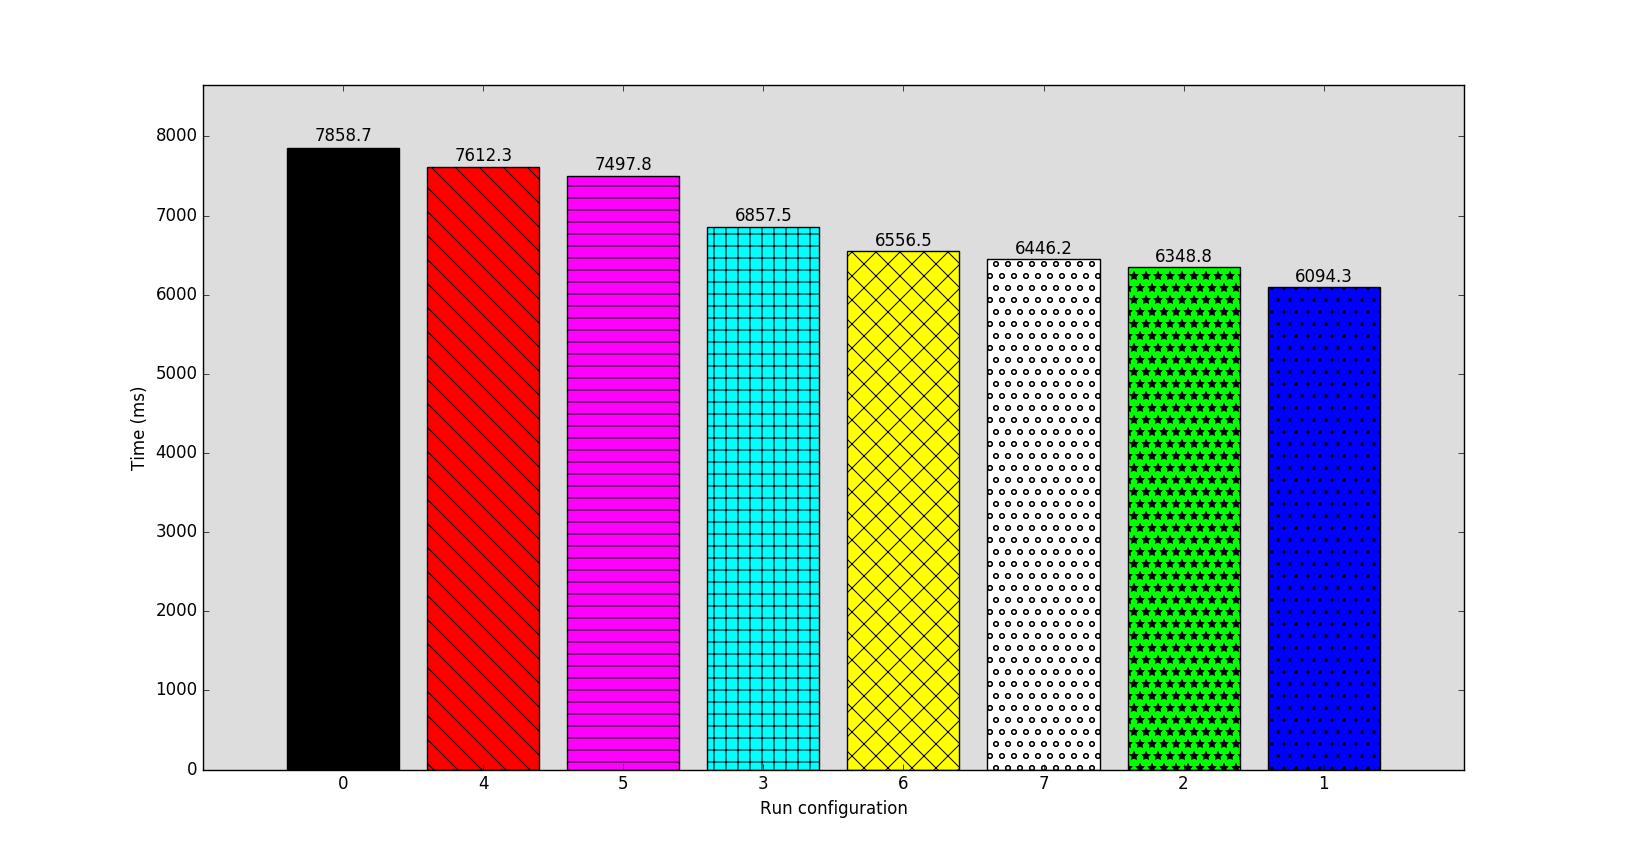
\includegraphics[width=0.9\paperwidth]{pythonthreading/images/initial_async_results}}
	\caption{Results of the initial experiment.}
	\label{fig:initial_results}
\end{figure}

To observe if Tribler can benefit from asynchrony, a simplistic yet representing experiment has been conducted.
An overview of the system this experiment was is available in Table~\ref{table:setup_initial_experiment}.
As Tribler functions as both a client and a server, CPU, I/O and network tasks are run interchangeably.
To mimic these workloads, the experiment has been set up as follows. 

First, as Tribler is both a client and a server, six client-server pairs are constructed where each server runs on a separate port.
Each pair has its own database containing two tables: one for the server to fetch data from and one for the client to insert data into. 
The table for the server to read from is filled with data beforehand.

Next, the client performs ten requests to the server, representing network traffic.
Upon receiving the request, the server performs a database query, generating I/O.
Unique queries are performed to avoid caching or other optimization techniques employed by the database engine that could bias the results.
Once the results have been fetched from the database, the server will perform several calculations on the data and compress the data using zlib, created a CPU-based load.
After that, the server returns the compressed data to the client upon which the client decompresses and parses it, generating additional CPU load.
Finally, the client will insert the data into the database generating additional I/O.

By measuring the time it takes for all client-serve pairs to complete the requests, we can measure the impact when performs one of the three different workloads synchronous versus asynchronous respectively.
In total there are eight possible configurations, defined in Table~\ref{tbl:experiment_configuration}.
The results of the experiment are visible in Figure~\ref{fig:initial_results}.
From this figure we conclude that offloading tasks to separate threads yield a superior performance over the synchronous case. Solely offloading I/O offers the best result: the time required to perform all requests decreased by 22.5\%.
As a Solid State Drive (SSD) was used in this experiment, it is possible that the performance gain when using a hard disk with moving parts would be bigger as read and write operations are slower on such disks.\\
Offloading all components using asynchronous programming results in a decrease of 18.0\% run time, 4.5\% less than only offloading I/O, which can be explained by the fact that the main thread is now mostly idle as all operations are offloaded to separate threads.\\
From these results we conclude that Tribler can benefit from asynchronous programming especially since I/O is the primary bottleneck.

\section{Conclusion}

In this chapter we analysed the python threading model in detail.
We explained why parallelism is not possible using standard Python and presented numerous initiatives that attempt to change this behaviour.\\
We investigated the performance behaviour of multi-threaded programs in Python and explained why multiple threads can cause performance regression.
Additionally, we have shown and repeated experiments conducted by David Beazley to confirm that this performance behaviour is still present in Python 2.7.\\
We shortly elaborated on the the new GIL introduced in Python 3.2, which could be a point of future work to improve Tribler's performance.
Next, we presented the use case of asynchrony in the context of I/O in Python and elaborated on its drawbacks.
Our initial experiment shows that we can indeed gain performance when using asynchrony, answering the second research question presented in Section~\ref{chp2:sct:objectives-research-questions}.